%%%%
\section{Fluorescência de Raios X}

Para determinação e quantificação das composição química (número atômico 
$ 10 < Z < 82$) das amostras foi utilizada a técnica não-destrutiva de 
\textbf{Fluorescência de Raios X (XRF)}.

\textbf{XRF} é um método analítico quali-quantitativo, 
multielementar, que mede os raios X característicos emitidos dos átomos da amostra, 
depois de também serem excitados por raios X. Não exige pré-tratamento químico
das amostras e permite análise simultânea dos elementos químicos.

Há basicamente 3 etapas envolvida na técnica de \textbf{XRF}:
excitação da amostra, emissão de raios x pelos átomos da amostra
e detecção. A excitação pode ocorrer por feixe de raios X (ou raios gamas) 
produzido em fontes radioativas, por partículas aceleradas ou 
por tubos geradores de raios x quando submetidos a diferença de potencial
\citep{jenkins1988}. 

O feixe de raios X incidente expulsa os elétrons das camadas mais 
internas $K$ e $L$, produzindo vacâncias. Para tal, a energia do feixe
incidente deve ser maior que a energia de ligação dos elétrons nessas camadas. 

Um átomo com vacância é instável e rapidamente elétrons das camadas 
mais externas preenchem as vacâncias, liberando energia e estabilizando o átomo.  

A figura \ref{fig:shimadzu_atomo} ilustra classicamente o que ocorre com
o átomo ao ser excitado.

\begin{figure}[H]
\begin{center} 
  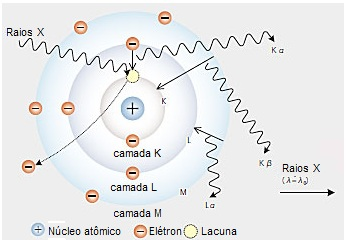
\includegraphics[width=0.5\textwidth]{../inputs/images/shimadzu_atomo.jpg}
  \caption{Ilustração clássica do fenômeno de fluorescência de raios X no átomo. 
           Figura acompanha o manual da \textbf{Shimadzu} do equipamento 
           \textbf{EDX 700} \label{fig:shimadzu_atomo}}
  % http://www.shimadzu.com.br/analitica/produtos/elemental/raios_x/eds/images/edx-7000_8000-2.jpg
\end{center}
\end{figure}

As transições dos elétrons entre o nível quântico $L$ e
$K$ liberam raios X característicos do átomo em questão. 

Transições da camada $L$ para $K$ são do tipo $K_{\alpha}$, de $M$ para $K$ 
são $K_{\beta}$ e de $M$ para $L$ são $L_{\alpha}$ ou $L_{\beta}$. 
As camadas $L$ e $M$ possuem ainda subníveis de energia, o que resulta em diversas
combinações de transições, sendo algumas transições proibidas, e outras 
com diferenças de energia indistinguíveis para os tipos de 
detectores utilizados.

A \textbf{notação de Siegbahn} \citep{jenkins1991} permite identificarmos 
melhor os subníveis de origen e destino. 
Por exemplo, a transição de $M_{IV}$ para $L_{III}$ é uma transição do 
tipo $L_{\beta_1}$, outras transições possíveis estão na figura \ref{fig:siegbahn}. 

\begin{figure}[H]
\begin{center} 
  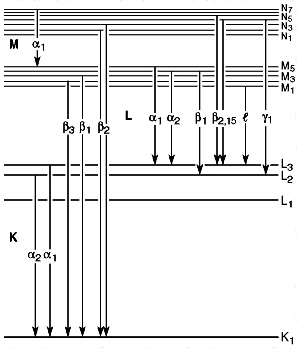
\includegraphics[width=0.5\textwidth]{../inputs/images/Siegbahn.jpg}
  \caption{Transições de elétrons entre os subníveis das camadas $K$, $L$ e $M$. 
           Figura extraída de \citep{jenkins1991} \label{fig:siegbahn}}
\end{center}
\end{figure}

Na prática, agrupa-se transições dos subníveis e trabalha-se com 
as denominações de linhas $K$ e $L$ apenas. 

%%%%
\subsection{Tipos de \textbf{XRF}}

Há diferentes tipos de equipamentos de \textbf{XRF} que se diferenciam 
como os raios x são detectados, os mais comuns são:

\begin{itemize}
  \item \textbf{ED-XRF}: fluorescência de raios X por dispersão em energia;
  \item \textbf{WD-XRF}: fluorescência de raios X por dispersão em comprimento de onda;
  \item \textbf{EDP-XRF}: fluorescência de raios X polarizada;
  \item \textbf{T-XRF}: fluorescência de raios X por reflexão total;
\end{itemize}

%TODO: explicar resumidamente cada um dos tipos de XRF 

A \textbf{XRF-ED} usa detectores de semicondutores capazes de
discriminar energias próximas. 
O detector mais empregado é o de silício ativado com lítio $Si(Li)$. 

A distinção dos fótons é feita pela amplitude do pulso 
eletrônico produzido no detector, pois os pulsos eletrônicos são
proporcionais às energias dos raios X incidentes. O sistema eletrônico do 
equipamento armazena o pulso em um multicanal.

%TODO: fazer esquema do ED-XRF igual http://usp.br/faepah/sites/default/files/Fluoresc%C3%AAncia%20de%20Raio%20X_1.jpg

Na \textbf{WD-XRF} os raios X da amostra atravessam um cristal 
e identifica-se os elementos químicos pelo o ângulo de difração $\theta$, segundo 
a \textbf{Lei de Bragg} \ref{eq:bragg}. 

\begin{equation}
  \label{eq:bragg}
  2d sen(\theta) = n \lambda
\end{equation}

Sendo $d$ a distância entre planos do cristal, $\theta$ o ângulo de incidência em 
relação ao plano considerado, $\lambda$ o comprimento de onda (e portanto a energia) 
da radiação incidente e $n$ um inteiro. 

%%%%
\subsection{\textbf{ED-XRF} do \textbf{LAPAt}}

Neste trabalho foi utilizado uma \textbf{ED-XRF} da marca \textbf{Shimadzu} 
modelo \textbf{EDX 720HS} \ref{fig:xrfed_iag} pertencente ao 
\textbf{Laboratório de Análise dos Processos Atmosféricos - LAPAt}
no \textbf{Instituto de Astronomia, Geofísica e Ciências Atmosféricas - IAG-USP}.

\begin{figure}[H]
\begin{center}
  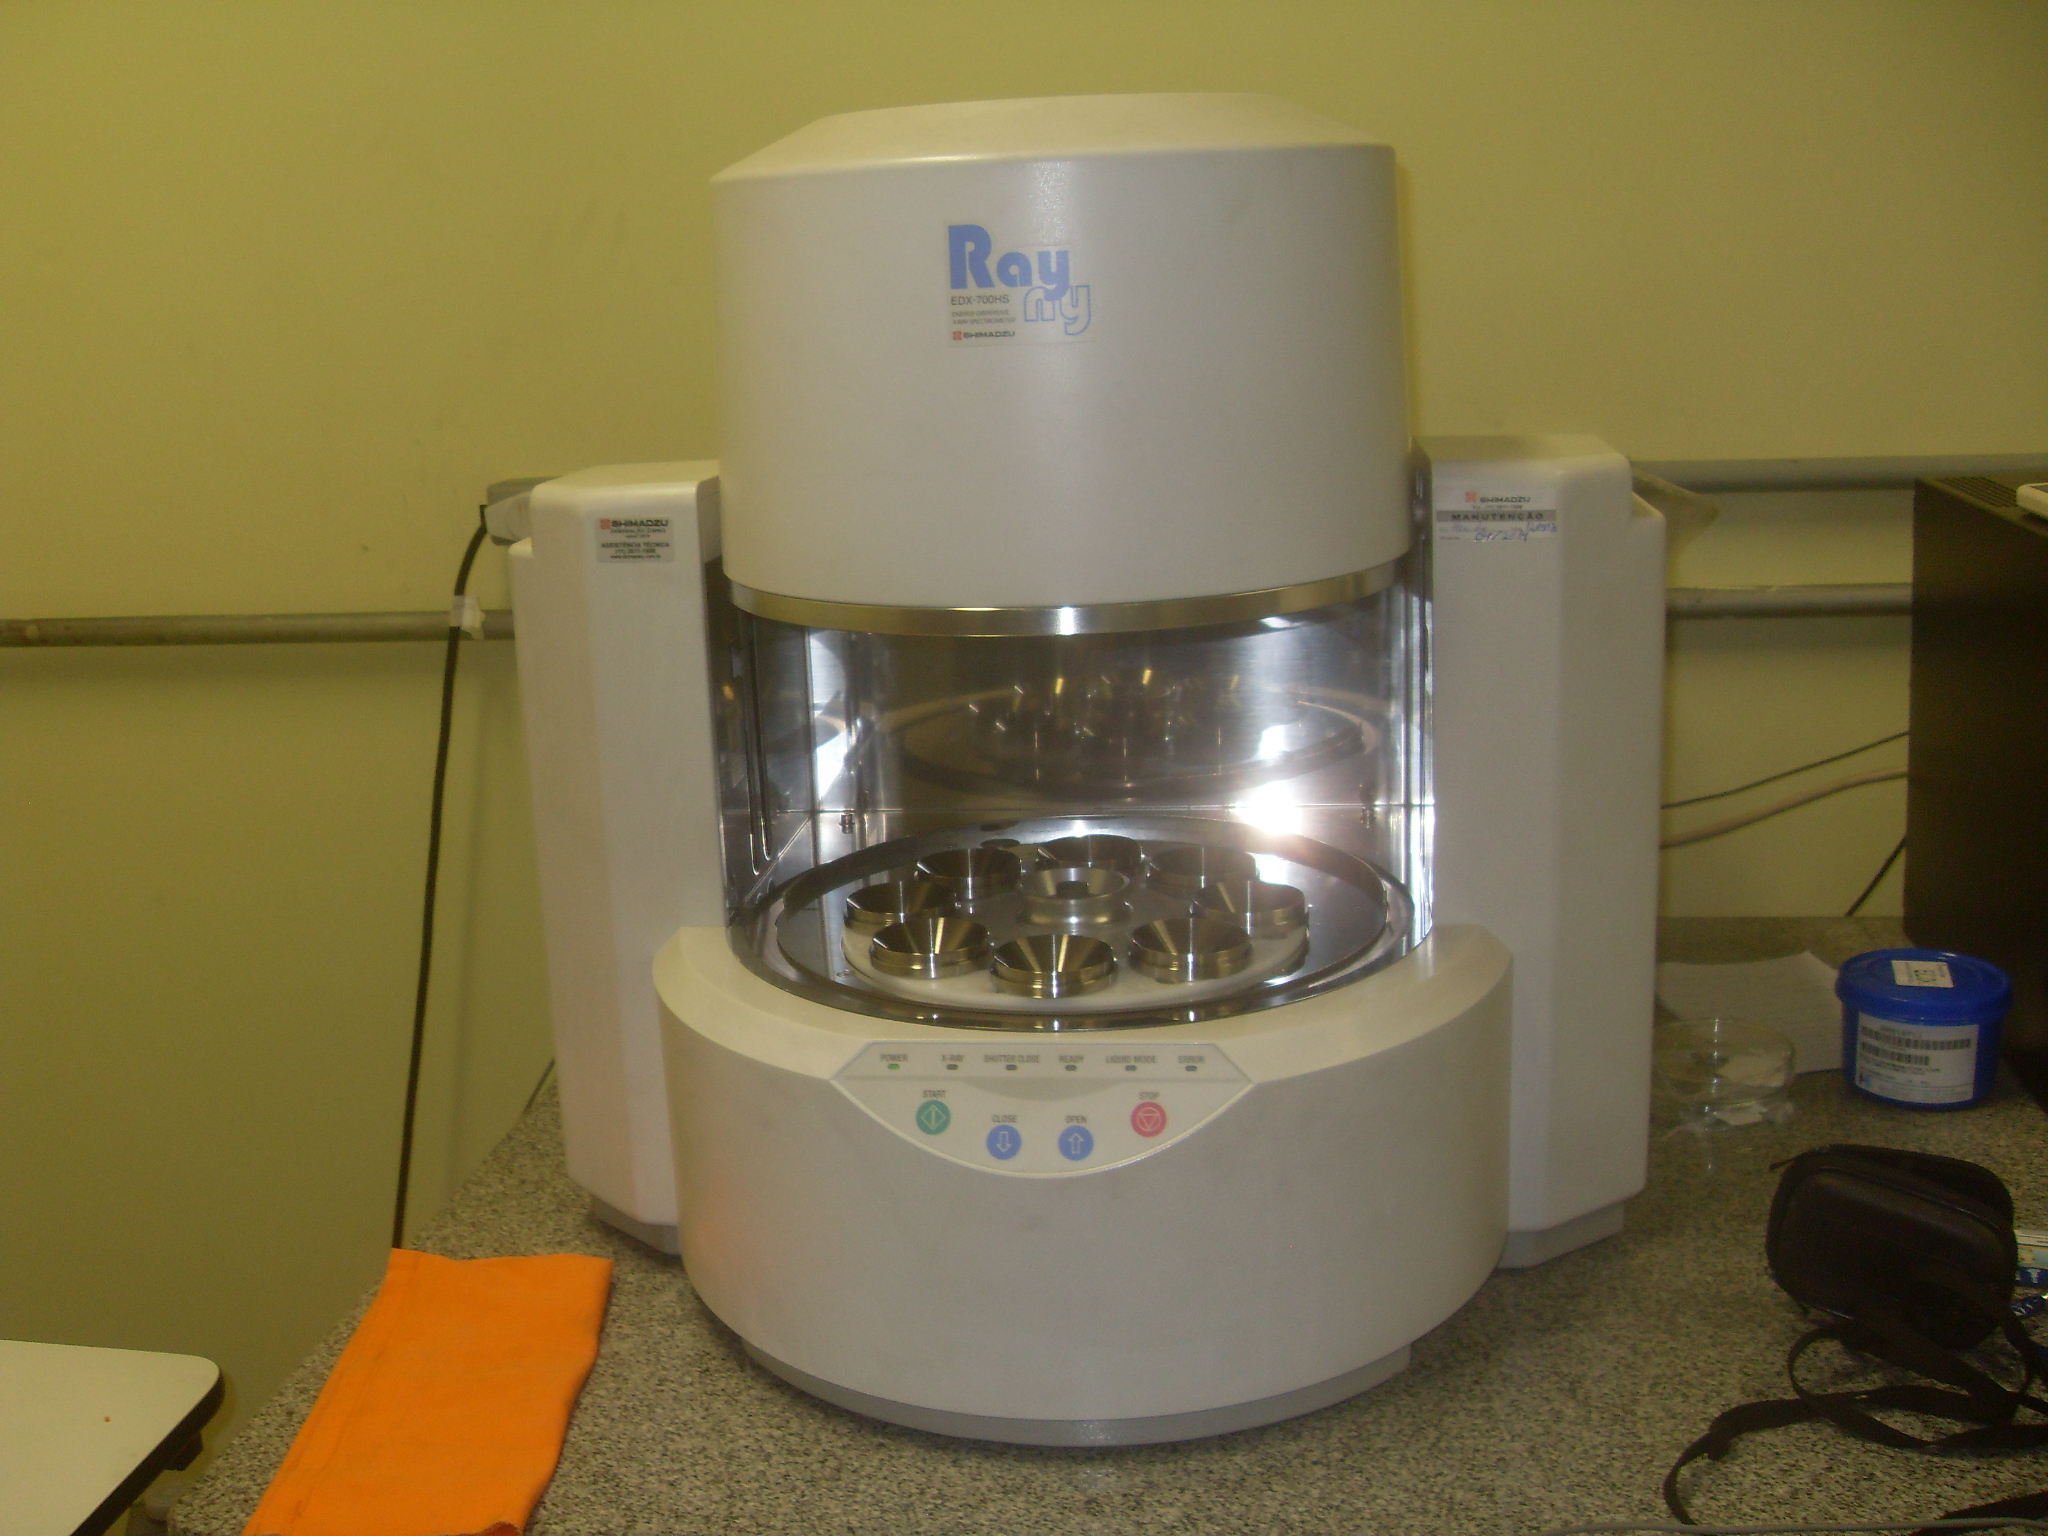
\includegraphics[width=0.5\textwidth]{../inputs/images/xrf-ed-IAG-USP.jpg}
  \caption{\textbf{ED-XRF Shimadzu 720HS} do \textbf{Laboratório de Análise dos Processos Atmosféricos - LAPAt} do
           \textbf{Instituto de Astronomia, Geofísica e Ciências Atmosféricas - IAG-USP} \label{fig:xrfed_iag}}
\end{center}
\end{figure}

Um tubo de ródio $Rh$ submetido a uma diferença de potencial 
de $50 kV$ foi utilizado para geração do feixe de raios X.
O detector de silício ativado com lítio $Si(Li)$ possui sensibilidade
para medida de $0$ a $20 keV$ e o sistema eletrônico conta com multicanal 
de 2048 canais.
Um filtro de alumínio $Al$ foi posto entre o feixe e a amostra para remover
a radiação da linha $L$ dos raios X do tubo de ródio, para melhorar o limite
de detecção dos elementos com energia menores que $2,6 keV$ (energia da linha
$L$ do feixe incidente).

Tipicamente, o tempo de irradiação de cada amostra foi $\pm 18$ minutos com 
13\% de tempo morto. Como as amostra estavam completamente carregadas, 
a corrente foi de 1000 $\mu A$. 

Na imagem \ref{fig:xrfed_software} extraída do software que acompanha o equipamento
\textbf{ED-XRF Shimadzu 720HS} pode-se verificar em tempo real características da
análise como: voltagem e corrente no tubo, filtro, informação se câmera está 
em vácuo ou não, dentre outros dados que ajudam o pesquisador a conferir se 
a análise está sendo realizada como planejada. 

\begin{figure}[H]
\begin{center}
  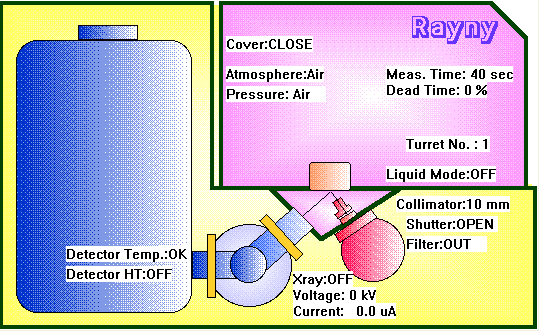
\includegraphics[scale=0.4]{../inputs/images/edx_iag_monitor.png}
  \caption{\textbf{ED-XRF Shimadzu 720HS}. Imagem gerada pelo software que 
           acompanha equipamento e mostra o status do mesmo. \label{fig:xrfed_software}}
\end{center}
\end{figure}

O \textbf{EDX 720HS} aceita carrossel de 8 ou 16 posições, mas o \textbf{LAPAt}
contava apenas com o carrossel de 16 posições, que não cabia os filtros de Teflon, 
usados nesta pesquisa, devido ao diâmetro. Assim, foi adquirido da \textbf{Shimadzu} 
o carrossel da figura \ref{fig:carrossel8} de 8 posições.

\begin{figure}[H]
\begin{center}
  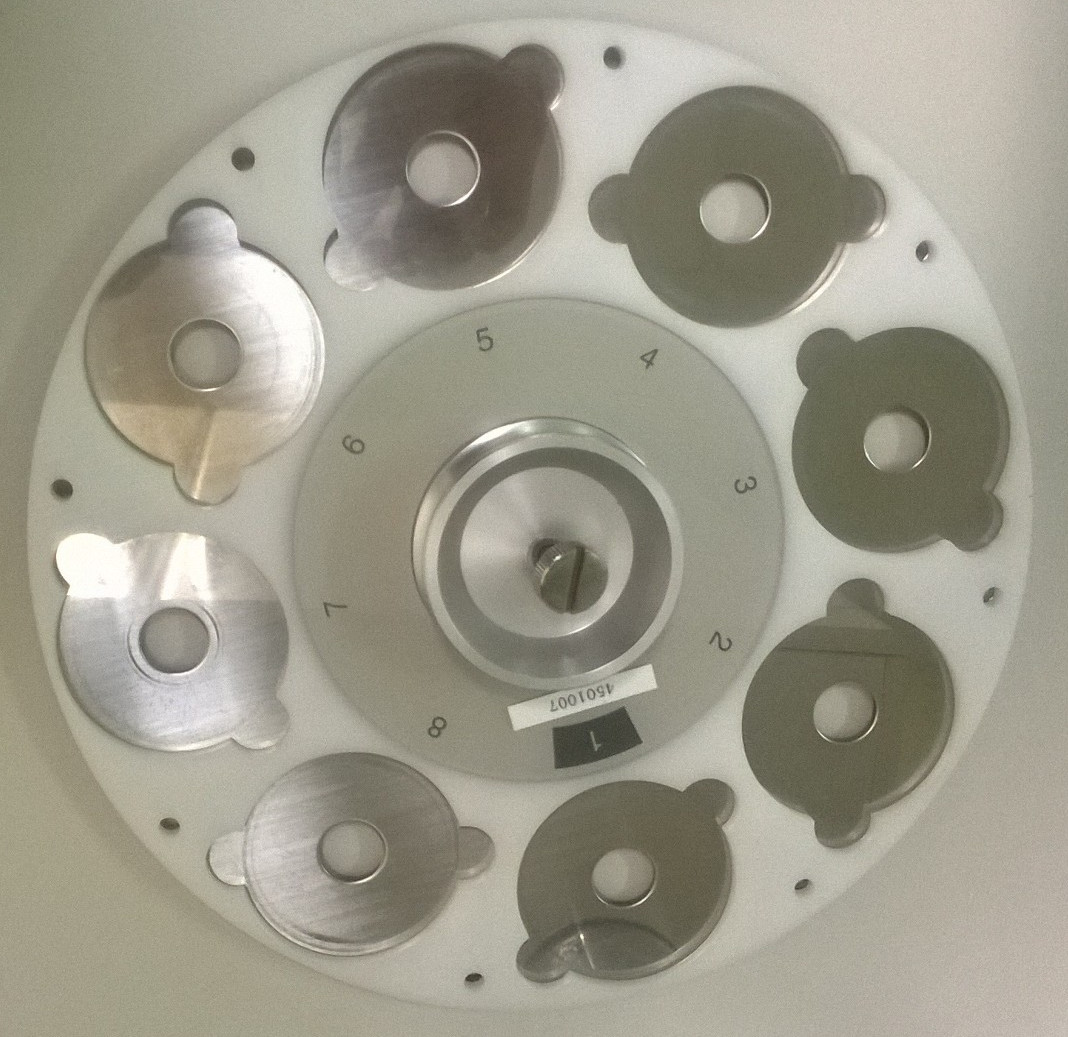
\includegraphics[width=0.7\textwidth]{../inputs/images/carrossel8.jpg}
  \caption{Carrossel de 8 posições para \textbf{ED-XRF Shimadzu 720HS} \label{fig:carrossel8}}
\end{center}
\end{figure}

Como a análise é feita em vácuo, foi necessário criar o suporte 
da figura \ref{fig:suporte8} que segurasse o filtro de Teflon no 
carrossel de 8 posições durante o vácuo. 
Os suportes de alumínio foram criados pela oficina do \textbf{Instituto de
Física da USP} e permitiram 

\begin{figure}[H]
\begin{center}
  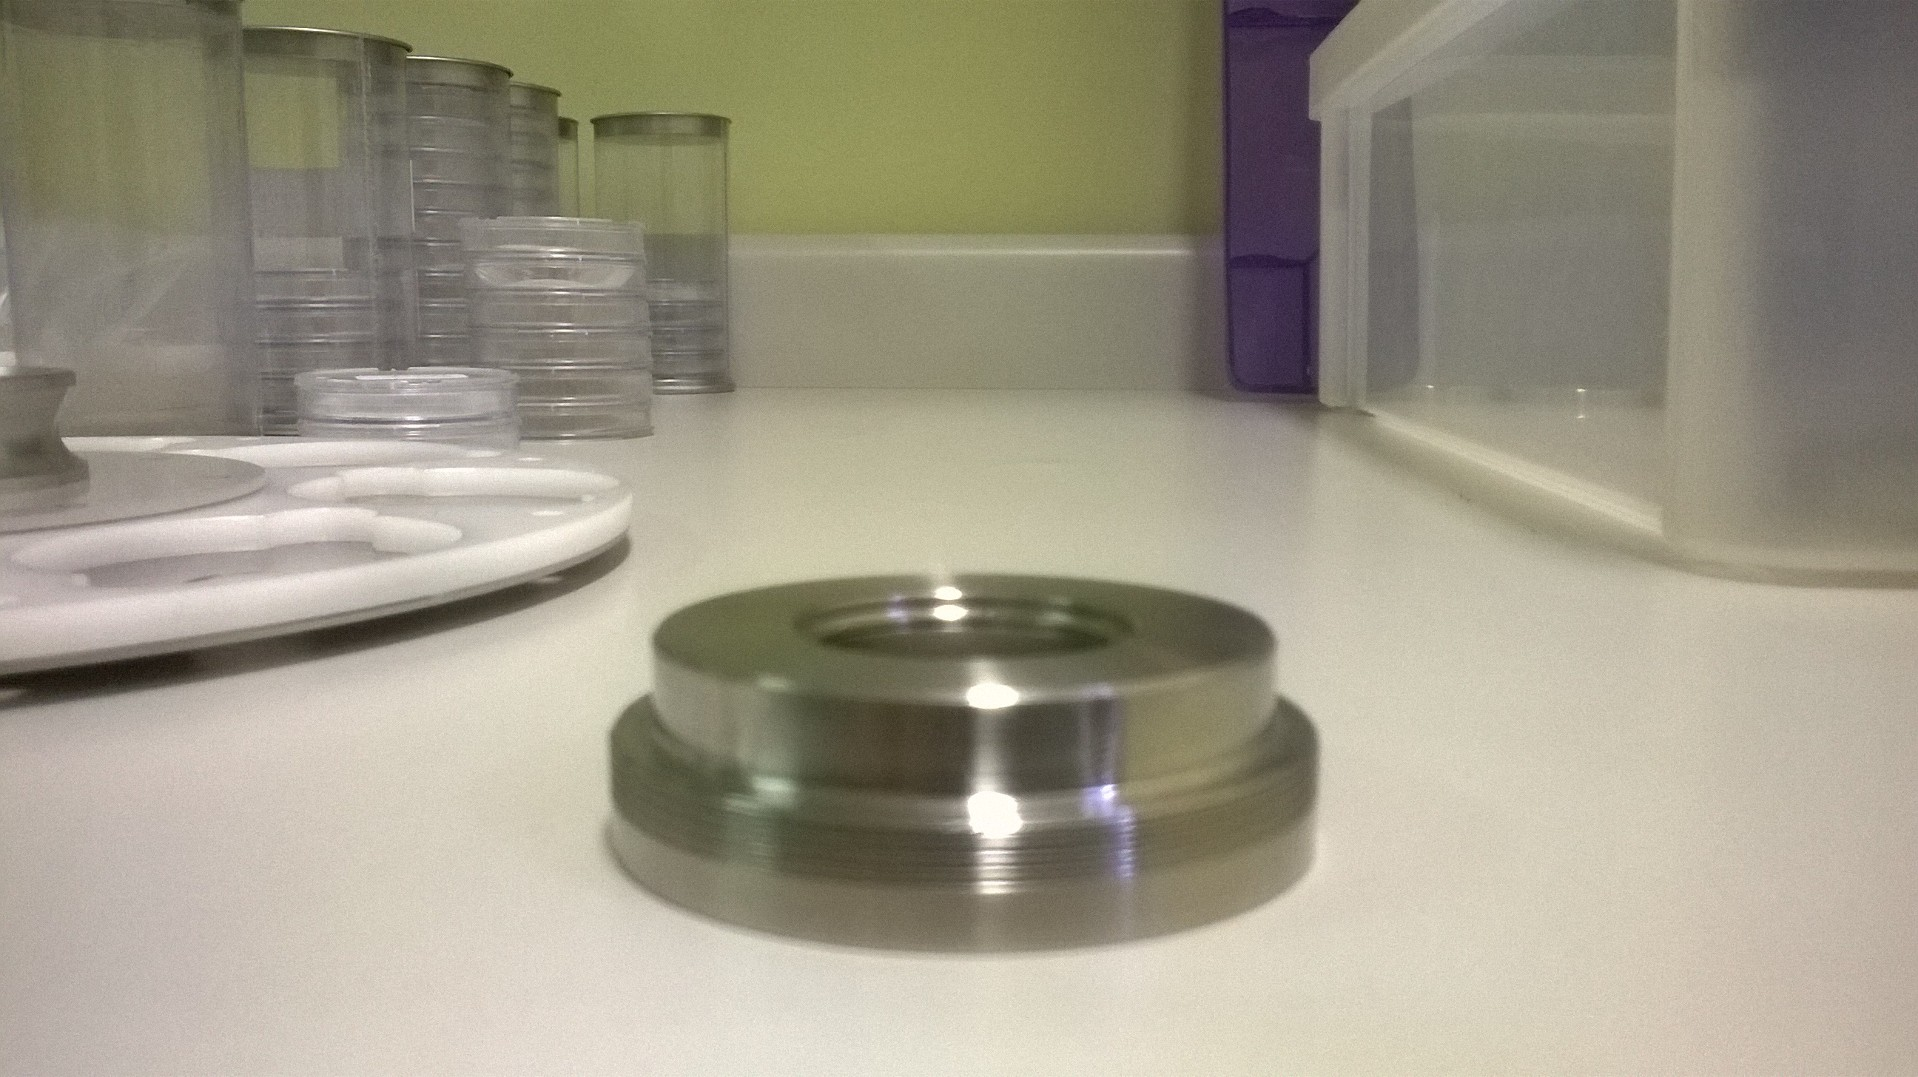
\includegraphics[width=0.5\textwidth]{../inputs/images/suporte8.jpg}
  \caption{Suporte desenvolvido para carrossel de 8 posições pela oficina
           do \textbf{Instituto de Física da USP} \label{fig:suporte8}}
\end{center}
\end{figure}

%%%%
\subsection{Calibração do \textbf{ED-XRF}}

Amostra espessas apresentam o efeito matriz, ou seja, interações dos 
raios X característicos com os elementos da amostras, causando 
absorção do raios X ou mesmo reforço de raios X. 
Para os filtros usados na amostragem, Teflon, será considerado filtro
fino, ou seja, fino o suficiente para desconsiderarmos o efeito matriz.

Alvos padrões, com densidade elementar conhecida, podem ser 
comprados ou produzidos, dependendo da precisão desejada.
Neste projeto foram comprados alvos padrões da \textbf{Micromatter}
com incerteza de 5\%. 
Não há alvos para todas espécies possíveis de se encontrar na atmosfera. 

Assim, usou-se um método de calibração proposto por \citep{tabacniks2000}
para sistema \textbf{PIXE (Particle Induced X-Ray Emission)} com pequenas
adaptações no contexto da \textbf{ED-XRF}.   
A calibração permitiu abrangência de todos elementos de número atômico 
$ 10 < Z < 83$ nas análises de \textbf{ED-XRF}. 
Desensolve-se ainda, uma metodologia para estimativa das incertezas
para a calibração.   

O \textbf{PIXE (Particle Induced X-Ray Emission)} é
outro método comumente usado em análises ambientais. 
Usa feixe de íons (prótons ou alfas) para excitação dos 
átomos das amostras.

\begin{figure}[H]
\begin{center} 
  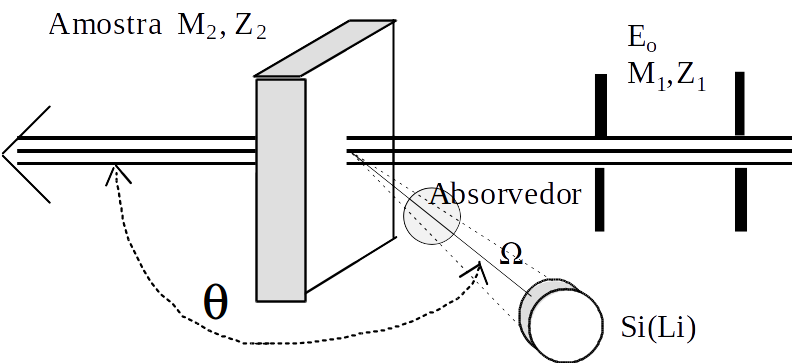
\includegraphics[width=0.7\textwidth]{../inputs/images/arranjopixe.png}
  \caption{Arranjo experimental básico para análise de método PIXE 
           \citep{tabacniks2000} \label{fig:arranjopixe}}
\end{center}
\end{figure}

Dado o arranjo experimental da figura \ref{fig:arranjopixe} e
considerando o filtro fino (alguns $\mu m$),
\citep{tabacniks2000} chega na equação \ref{eq:npixe} para 
quantidade de raios X $N$ contadas no detector. 

\begin{equation}
  \label{eq:npixe}
  N(Z) = \frac{\Omega}{4\pi} \sigma \zeta T t_z \frac{Q}{qe}
\end{equation}

Sendo $Z$ a espécie química, o número de raios X detectados 
$N(Z)$ é proporcional à densidade (massa ou átomos por área) $t_Z$ 
e a carga coletada $Q$.
$\zeta$ é a eficiência do detector, $\sigma_x$ é a secção de choque, 
$\Omega$ é o ângulo sólido, $T$ é a transmitância para raios-X em 
caso de uso de absorvedores (colocados entre a amostra e o detector), 
$q$ é o estado de carga da partícula incidente e 
$e$ é a carga do elétron \citep{tabacniks1983}.

Para resolver a equação \ref{eq:npixe}, parâmetros do arranjo experimental
($\Omega$, $\sigma$, $\zeta$ e $T$) deveriam ser conhecidos. 

Na prática, é mais comum é irradiar alvos de calibração com $t_z$ conhecidos,
e encontrar uma variável única proporcional aos parâmetros do arranjo experimental.
Da-se o nome de fator de resposta $R(Z)$ a essa variável.

Assim, adaptando a nomenclatura da equação \ref{eq:npixe} para o contexto 
da \textbf{ED-XRF} e incluindo o fator de resposta $R(Z)$ chegamos na equação 
\ref{eq:contagem}.

\begin{equation}
  \label{eq:contagem}
  N(Z) = R(Z) I\Delta t \frac{m(Z)}{A}
\end{equation}

$R(Z)$ é o fator de resposta, $I\Delta t$ é a carga efetiva expressa
em termos da corrente e do tempo efetivo de análise.
A densidade $t_z$ está representada pela razão da massa $m(Z)$ pela 
área de deposição $A$.

Isolando-se $R(Z)$ em \ref{eq:contagem} obtém-se a equação para cálculo 
do fator de respota \ref{eq:fator_de_resposta}.
Irradiando-se alvos padrões - que possuem densidades $m(Z)/A$ conhecidas - 
mede-se $N(Z)$ e $I \Delta t$. Assim, são calculados fatores de repostas $R(Z)$ 
para os respectivos alvos padrões. 

\begin{equation}
  \label{eq:fator_de_resposta}
  R(Z) = \frac{N(Z) A}{m(Z)I \Delta t}
\end{equation}

Considerando que a incerteza da corrente e do tempo vivo são
desprezíveis perto da incerteza da massa, da contagem e da área, 
a incerteza do fator de resposta pode ser calculada usando a expressão
de propagação de erro para variáveis independentes conforme equação 
\ref{eq:erro_fator_de_resposta}.

\begin{equation}
  \label{eq:erro_fator_de_resposta}
  \sigma_{R(Z)}^2 = {R(Z)}^2 \left( \left(\frac{\sigma_{N(Z)}}{N(Z)}\right)^2 + 
                                  \left(\frac{\sigma_A}{A}\right)^2 + 
                                  \left(\frac{\sigma_{m(Z)}}{m(Z)}\right)^2 
                             \right)
\end{equation}

Dados ambientais são reportados em medidas de concentração,
razão da massa $m(Z)$ pelo volume amostrado ($\mu g/m^3$).
Conhecendo-se o fator de resposta $R(Z)$, pode-se calcular a massa $m(Z)$ 
pela equação \ref{eq:xrfedmassa}, que nada mais é que o isolamento de $m(Z)$ na 
\ref{eq:contagem}. 

\begin{equation}
  \label{eq:xrfedmassa}
  m(Z) = \frac{N(Z) A}{ R(Z)I \Delta t}
\end{equation}

Empregando-se novamente a expressão da propagação de erro para variáveis independentes, 
a incerteza na massa pode ser calculada pela equação \ref{eq:erro_massa}.

\begin{equation}
  \label{eq:erro_massa}
  \sigma_{m(Z)}^2 = {m(Z)}^2 \left( \left(\frac{\sigma_{N(Z)}}{N(Z)}\right)^2 + 
                                  \left(\frac{\sigma_A}{A}\right)^2 + 
                                  \left(\frac{\sigma_{R(Z)}}{R(Z)}\right)^2 
                             \right)
\end{equation}


Entretanto, para cada espécie química de interesse, seria necessário 
o alvo de calibração correspondente.

Nem sempre é possível adiquirir alvos de calibração para todos elementos
químicos e a incerteza garantida pela \textbf{Micromatter}) é de 5\%. 

No gráfico da figura \ref{{fg:edxrfcalib2010maio}} estão plotados os $R(Z)$ 
dos alvos padrões da \textbf{Micromatter} irradiados em Maio de 2010. 

\begin{figure}[H]
  \begin{subfigure}[b]{0.45\textwidth}
    \includegraphics[width=\textwidth]{../outputs/plot_R_maio2010K.pdf}
    \caption{Linha K}
  \end{subfigure}%
  \begin{subfigure}[b]{0.45\textwidth}
    \includegraphics[width=\textwidth]{../outputs/plot_R_maio2010L.pdf}
    \caption{Linha L}
  \end{subfigure}
  \caption{Fatores de respostas $R(Z)$ dos para alvos padrões da 
           \textbf{Micromatter} irradiados em Maio de 2010. 
           \label{fg:edxrfcalib2010maio}}
\end{figure}

Nota-se que é possível fazer um ajuste polinomial nos dados, o que 
permite encontrar $R$ para elementos que não possuem alvos padrões.

%%%%
\subsection{Estimativa do erro}

Utilizou-se o \textbf{Ajuste dos Mínimos Quadrados Matricial} 
para a estimativa do erro do ajuste \citep{helene2006}.

Dada as variáveis $Y_i$ e $X_i$ relacionadas polinomialmente, 
conforme \ref{eq:polinomio}.

\begin{equation}
  \label{eq:polinomio}
  \begin{split}
    y_1 = a + b x_1 + c{x_1}^2 + d{x_1}^3 + ...\\
    y_2 = a + b x_2 + c{x_2}^2 + d{x_2}^3 + ... \\
    ...
  \end{split}
\end{equation}

A representação matricial da equação \ref{eq:polinomio} pode 
ser escrita como \ref{eq:polinomioMatriz}.

\begin{equation}
  \label{eq:polinomioMatriz}
  [Y] = [A][X]
\end{equation}

Os coeficientes ajustados $[Ã]$ são dados pela equação \ref{eq:coeficientesajustados},
que depende da matriz de covariância dos coeficientes $[V_{Ã}]$, 
dada pela equação \ref{eq:matrizcovariancia}.

\begin{equation}
  \label{eq:coeficientesajustados}
  [Ã] = [V_{Ã}] ([X]^T {[V_Y]}^{-1} [Y])
\end{equation}

\begin{equation}
  \label{eq:matrizcovariancia}
  [V_{Ã}] = ([X]^T [V_Y]^{-1} [X])^{-1}
\end{equation}

Com o coeficientes ajustados $[Ã]$ pode-se calcular os 
$[\tilde{Y}]$ ajustado \ref{eq:polinomioajustado}.

\begin{equation}
  \label{eq:polinomioajustado}
  [\tilde{Y}] = [Ã][X]
\end{equation}

Por fim, a incerteza é dada pela diagonal da matriz de covariância 
de $[\tilde{Y}]$, $[V_{\tilde{Y}}]$ em \ref{eq:matrizcovarianciaY}.

\begin{equation}
  \label{eq:matrizcovarianciaY}
  [V_{\tilde{Y}}] = [X] [V_{Ã}]^{-1} [X]^{-1}
\end{equation}

Adaptando-se para nosso contexto, $[Y]$ será os fatores de respostas $[R]$,
e $[X]$ os números atômicos $[Z]$.

%%%%
\subsection{Limite de Detecção}

O limite de detecção é o valor mínimo de massa que a amostra precisa
ter para ser detectada pelo \textbf{ED-XRF}. 

Irradiando-se uma amostra branca obtém-se o número de contagens medidas ($N_B$) 
sob o pico dos elementos que se quer calcular o limite de detecção. 

A medida do detector segue uma \textbf{distribuição de Poisson}
pois realiza contagens aleatórias em torno do valor médio da energia 
no pico. O desvio padrão da contagem $N$ é portanto $\sqrt{N}$.

\begin{equation}
  \label{eq:limitedeteccao}
  N_{LD} = 3 x \sqrt{N_B}
\end{equation}

O número mínimo de contagens para se distiguir um pico é $N_{LD}$ e é
calculado usando \ref{eq:limitedeteccao}.
Pode-se calcular o limite de detecção em termos da massa 
elementar usando \ref{eq:xrfedmassa}. 

O limite de detecção muda conforme a quantidade de material coletado, podeaqui fizemos um filtro supercarregado
e outro branco. O branco seria o menor LD possível para esse tipo de filtro Teflon. 
O LD muda se mudar o tipo de filtro: material e espessura , pois muda o NB. 

Lembrete, usa-se LD K do sódio até Mo. E L para frente do Mo.  
  

No caso das concentrações diárias, obtidas por EDX.  

Os valores faltantes foram preenchidos com o valor da metade do Limite de Detecção 
(LD/2, supondo que a concentração não detectada de um elemento que aparece 
frequentemente nas demais amostras esteja entre 0 e LD, com igual 
probabilidade de ocorrência para cada valor, LD/2 seria a média e, portanto, 
o valor mais provável entre estes valores "invisíveis"); 

para sua incerteza tomou-se 5LD/6 \citep{polissar1998}.


Densidade mínima para haver detecção da espécie. % como determina para XRF?




%%%%
\subsection{WinQxas – Quantative X-Ray Spectra Analysis System}

O WinQxas foi o programa utilizado para integração dos espectros obtidos no \textbf{ED-XRF}. 

Ele foi elaborado sob o patrocínio da Agência Internacional de Energia Atômica (IAEA), por um grupo chefiado pelo Profº. Dr. P. Van Espen da Universidade de Antuérpia, Bélgica entre 1987 a 1994, e reformulado para acompanhar as necessidades laboratoriais atuais, como banco de dados mais atualizados e compatibilidade com novos sistemas operacionais. 
Realizamos a integração de todos os espectros (exemplo na Fig.9), através desse programa, para estimar a composição elementar do MP2,5. Para tanto, o sistema também foi  calibrado, a partir de amostras padrões, com concentrações definidas. Os parâmetros iniciais para o ajuste de energia, por mínimo Chi quadrado, foram determinados  a partir de espectros com picos bem definidos. Obtém-se, assim, os parâmetros iniciais de uma relação linear entre canal e energia, bem como a relação abaixo, entre a largura do pico a meia altura (FWHM), com o nível geral de ruido (NOISE)  no espectro e um termo (FANO), dependente da energia (E):

%FWHM^2 = NOISE^2 + 2,35 x FANO  x E

%\begin{figure}[H]
%\begin{center}
%  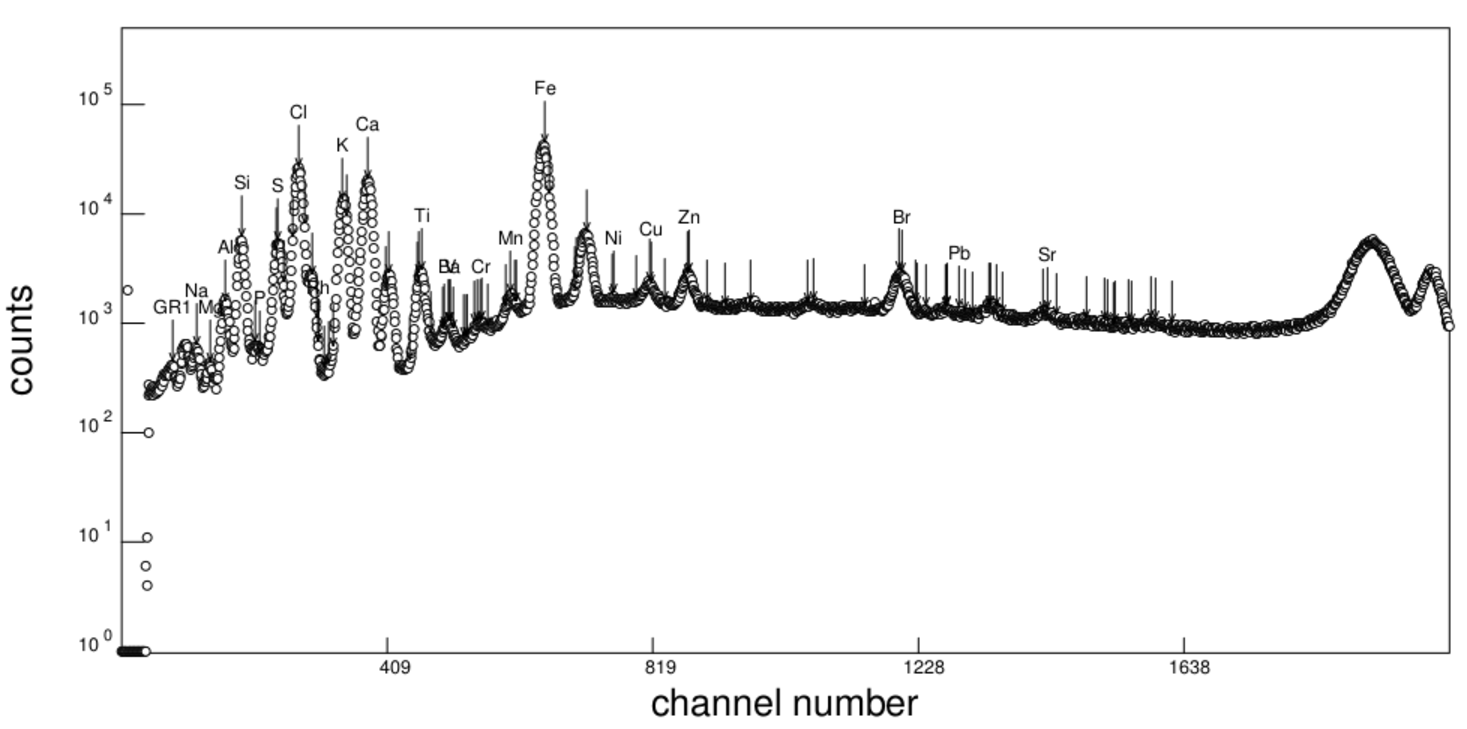
\includegraphics[scale=0.30]{../inputs/images/winqxas/GHA41editado.pdf}
%  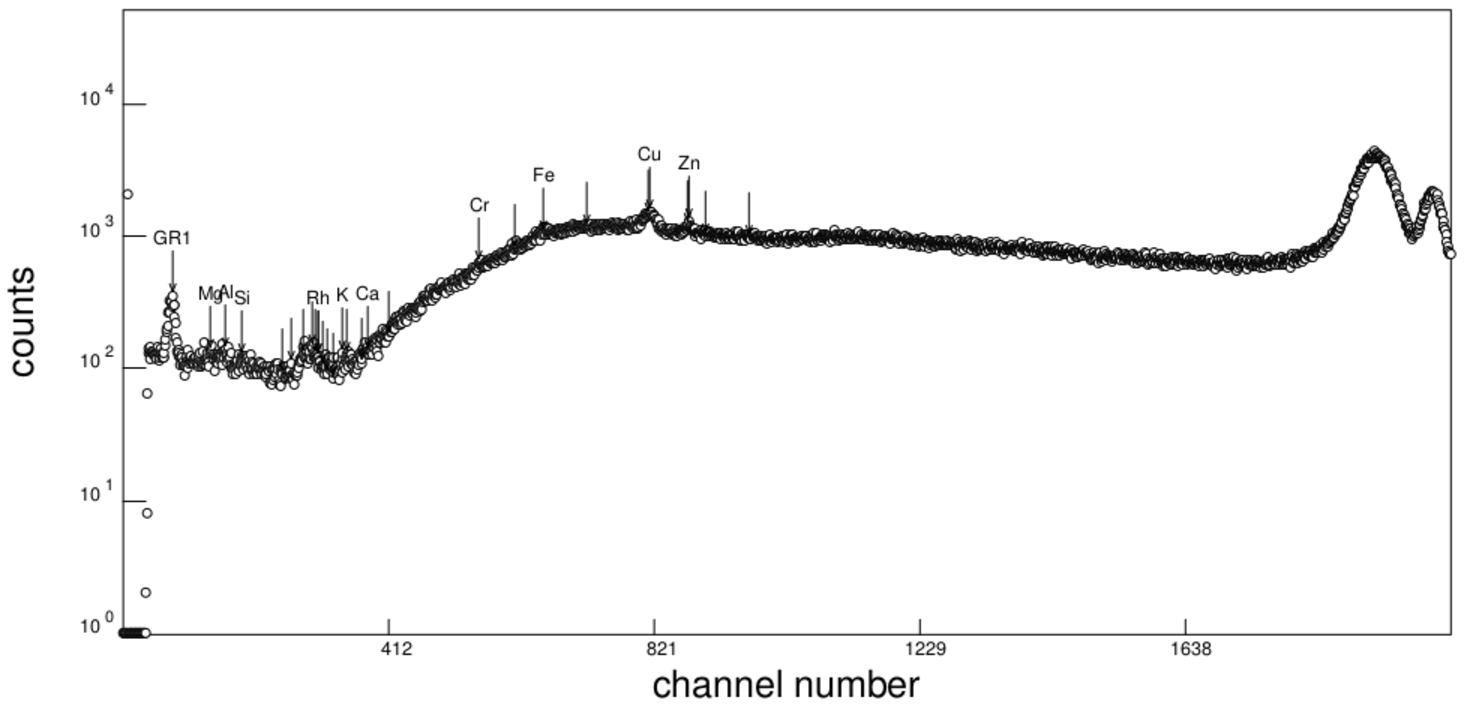
\includegraphics[scale=0.30]{../inputs/images/winqxas/GPE770editado.pdf}
%\end{center}

Este gráfico representa o número de contagens  versus a Energia (Kev) dos 	fótons vindos da amostras e recebidos pelo detector do EDX. Os picos 	característicos de elementos químicos encontrados estão indicados na figura.

O fundo do espectro dificulta a distinção dos picos e piora
o limite de detecção. É gerado pela radiação emitida pelo tubo de ródio
devido a aceleração e desaceleração de elétrons.

%%%%
\subsection{Fontes de erro no branco}


%TODO: Colocar espectro plot 

A análise dos espectros obtidos por esses métodos foram feitas no software WinQxas (IAEA, 2002).

A massa depositada no filtro amostrado $m(Z)_{medido}$ para um certo 
elemento $Z$, é composta pela massa coletada na amostragem $m(Z)$ 
mais a massa do filtro branco $m_{B}(Z)$. 

Um conjunto de 10 amostras brancas (campo e laboratório) foram analisadas, 
para eliminação da contaminação dos próprios filtros, assim como de 
transporte e manipulação.

A equação \ref{eq:contagem} pode ser escrita para representar essa situação
\ref{eq:contagem_medida}. 

\begin{equation}
  \label{eq:contagem_medida}
  N(Z)_{medido} = R(Z) I\Delta t \left( \frac{m(Z)}{A} + \frac{m_B(Z)}{A} \right)
\end{equation}  

Escrevendo a equação \ref{eq:contagem} para os brancos temos \ref{eq:contagembranco}:

\begin{equation}
  \label{eq:contagembranco}
  N_B(Z) = R(Z) I_B\Delta t_B \frac{m_B(Z)}{A}
\end{equation}

Isolando-se $m_B(Z)$ em \ref{eq:contagembranco} e substituindo em 
\ref{eq:contagem_medida}, encontramos \ref{eq:contagemcorrigida}:
 
\begin{equation}
  \label{eq:contagemcorrigida}
  N(Z) = N(Z)_{medido} - I\Delta t \left( \frac{N_B}{I_B \Delta t_B} \right)
\end{equation}


A incerteza da equação \ref{eq:contagemcorrigida}:

\begin{equation}
  \label{eq:erro_contagemcorrigida}
  \sigma_{N(Z)}^2 = \sigma_{N(Z)_{medido}}^2 + \left( \frac{I \Delta t}{I_B \Delta t_B} \right)^2 \sigma_{N_B}^2
\end{equation}



Quando se tem N alvos brancos, a concentração do elemento 
considerado será a média sobre os N dados e o desvip padrão $\sigma_p$.

Mas quando N<10 é pequeno, precisa haver um fator de correção conforme tabela.

\begin{table}[H]
\centering
\caption{My caption}
\label{my-label}
\begin{tabular}{ll}
N  & Fator \\
2  & 1,84  \\
3  & 1,32  \\
4  & 1,20  \\
5  & 1,14  \\
6  & 1,12  \\
7  & 1,11  \\
8  & 1,09  \\
9  & 1,08  \\
10 & 1,06  \\
20 & 1,03 
\end{tabular}
\end{table}

%Já o erro da integração do espectro é calculado pelo erro na integração de cada espectro de branco e, obviamente, tem que ser calculado sem branco, só com o fator de resposta (ou seja, a rotina que calcula a concentração tem que ser igual para o alvo comum e para o branco; mas o alvo comum tem que ter uma complementação no cálculo para subtrair o branco e adicionar o erro, devido ao branco). Havendo N alvos brancos, com erro  i de integração para cada um deles, o erro transferido para a média deve ser:

Temos duas fontes possíveis de erro.

1) Erro estatístico. Quando se tem N brancos, a concentração do elemento considerado será a média sobre os N dados. O erro será o desvio padrão (p não é o desvio padrão da média), porque é a chance de termos esse erro em cada filtro analisado e não sobre a média. Para considerar o sentido do desvio padrão (68,3\% de chance de pertencer ao amostral) ainda precisa haver um fator de correção quando N for pequeno. Seria bom corrigir para N<=10. Dai em diante pode usar fator 1, porque a correção seria pequena.

%$\sigma_{pc} = fatorr x \sigma_p$

2) Erro da integração do espectro. Esse erro é calculado pelo erro na integração de cada espectro de branco e, obviamente, tem que ser calculado sem branco, só com o fator de resposta (ou seja, a rotina que calcula a concentração - em µg/cm - tem que ser igual para o alvo comum e para o branco; mas o alvo comum tem que ter uma complementação no cálculo para subtrair o branco e adicionar o erro, devido ao branco). Havendo N alvos brancos, com erro  i de integração para cada um deles, o erro transferido para a média deve ser:

%\sigma_e = \sqrt{\frac{\Sigma \sigma_i}{N} }

3) Erro total no branco. O erro final em cada elemento do branco é obtido considerando que 1 e 2 (acima) são independentes, logo:

%$\sigma_{r} = \sqrt{\sigma_e^2 + \sigma_pc^2} $




